%%%%%%%%%%%%%%%%
%%  Template for latex documents
%%  Author: Marco A. Aquino-Lopez
%%  Nota: to get a word document use pandoc
%%  pandoc -f latex Articulo.tex -o Articulo.docx --bibliography=bibliography.bib
%%%%%%%%%%%%%%%%%
\documentclass [11pt] {article}
\usepackage [utf8] {inputenc}
%\usepackage[spanish]{babel}
\decimalpoint
\usepackage {graphicx}
\usepackage {amsfonts}
\usepackage {amsthm}
\usepackage {amsmath}
\usepackage {natbib}
\usepackage[in]{fullpage} %To have more in the page
%.____         ___________    ____  ___ 
%|    |   _____\__    _______ \   \/  / 
%|    |   \__  \ |    |_/ __ \ \     /  
%|    |___ / __ \|    |\  ___/ /     \  
%|_______ (____  |____| \___  /___/\  \ 
%        \/    \/           \/      \_/ 

\graphicspath{{Figures/}} %Setting the graphicspath

%Extra packages
\usepackage{placeins}

%%%%%%

\date{ }
\usepackage{color}

%%%% To mark notes or added text by Author1 (a1)
%%%% This allows to add notes
%\newcommand{\a1}{\color{red} }  %% begin
%\newcommand{\1a}{ \color{black}} %% end
%\newcommand{\cuta1}[1]{\ac [cut] \ca} %% to mark cut text
%\newcommand{\notea1}[1]{\textcolor{red}{(note)}\footnote{\ac #1 \ca}}  %% To add a note or comment

% NOTE: To produce blinded version, replace "0" with "1" below.
\newcommand{\blind}{1}
\newcommand{\papertitle}{Using $^{210}Pb$ Simulations for model Comparison and analysing}

\begin{document}
	\def\spacingset#1{\renewcommand{\baselinestretch}%
		{#1}\small\normalsize} \spacingset{1}
	%%%%%%%%%%%%%%%%%%%%%%%%%%%%%%%%%%%%%%%%%%%%%%%%%%%%%%%%%%%%%%%%%%%%%%%%%%%%%%
	\if1\blind
	{
		\title{\textbf{\papertitle}}

		\author{Marco A Aquino-L\'opez\thanks{
				Centro de Investigaci\'on en Matem\'aticas (CIMAT),
				Jalisco s/n, Valenciana, 36023 Guanajuato, GT, Mexico.
				email: \texttt{aquino@cimat.mx} } \thanks{Corresponding author.}
					\and
			Nicole K. Sanderson\thanks{
				College of Life and Environmental Sciences, University of Exeter,
				Exeter, EX4-4QJ.
				email: \texttt{N.K.Sanderson@exeter.ac.uk}}
					\and
			Maarten Blaauw\thanks{School of Natural and Built Environment,
				Queen's University Belfast,
				Belfast, BT7-1NN.
				email:\texttt{maarten.blaauw@qub.ac.uk}  }
					\and
			J Andr\'es Christen\thanks{
				Centro de Investigaci\'on en Matem\'aticas (CIMAT),
				Jalisco s/n, Valenciana, 36023 Guanajuato, GT, Mexico.
				email: \texttt{jac@cimat.mx}  }
			}
		\maketitle
	} \fi

	\if0\blind
	{
		\bigskip
		\bigskip
		\bigskip
		\begin{center}
			{\LARGE\bf \papertitle}
		\end{center}
		\medskip/
	} \fi

	\bigskip
\begin{abstract}
	To understand changes in peat accumulation in response to recent and rapid climate or anthropogenic change, accurate ages for the last 100-200 years are essential. Dating this period is often complicated by poor resolution and large errors associated with calibrating radiocarbon (14C) ages. The use of lead-210 ($^{210}Pb$) is a popular method as it allows for the measurement of absolute and continuous dates for the last ~150 years of peat accumulation. 
In ombrotrophic peatlands, the lead-210 dating method has traditionally relied on the Constant Rate of Supply (CRS) model which uses the radioactive decay equation to provide a logarithmic model to approximate dates, resulting in a restrictive model. Key limitations of the CRS model are: (1) the accurate assessment of the supported lead which varies between sites and can be problematic if sampling of the total inventory is not continuous (e.g. interval measurements, lack of sample); (2) the inconsistent estimation of uncertainties. The Plum model was developed in a statistical framework with a Bayesian approach, notably resulting in longer chronologies, more realistic uncertainty estimations, and has the advantage of not double-modelling dates for final age-depth models, primarily radiocarbon and 210Pb chronologies. 
Here, we present two thorough tests of Plum. First, we created scenarios using simulated datasets with known age-depth functions in a range of shapes and with varying sampling resolution. These simulations are created using the physical behavior that most 210Pb dating models are based on. Plum and CRS model outputs are compared under each scenario. We also take this opportunity to demonstrate the new Plum’s R package, for use by non-statisticians in palaeoecological studies. We also compare the lead-210 dates derived from CRS models and from Plum using real peat cores with additional independent dating controls from Eastern Canada. These cores represent a thorough test for Plum, as permafrost thaw drastically changes stratigraphy and peat type (e.g. shift from ligneous peat to Sphagnum moss) which affects 210Pb retention within the peat. Recent decadal-scale changes are still poorly represented so accurate dating is now essential to quantify changes in carbon accumulation rates and predict future trends.
\end{abstract}
	\noindent%
	{\it Keywords:} Chronology, Constant Rate of Supply, Plum, Simulations.
	\vfill
	\newpage
	\spacingset{1.45} % DON'T change the spacing!

%%%%%%%%%%%%%%%%%%%%%%%%%%%%%%%%%%%%%%%%%%%%%%%%%%%%%%%%%%%%%
%%%%%%%%%%%%%%%%%%%%%%%%%%%%%%%%%%%%%%%%%%%%%%%%%%%%%%%%%%%%%
\section{Introduction}



\section{Simulations}
	In order to observe the accuracy and precision of any model we need data to which we know the true age-depth function. \citet{Blaauw2018} presented a methodology for simulating radiocarbon dates and as their uncertainty, on the other hand \citet{Aquino2018} presented an approach for simulating $^{210}Pb$ data given a age-depth function $f(t)$, it is important to note that this simulations follow the equations presented by \citet*{Appleby1978,Robbins1978}. By using the approach presented by \citet{Aquino2018} for obtaining $^{210}Pb$ simulated data from and the uncertainty estimations presented by \citet{Blaauw2018}, we can obtained resalable $^{210}Pb$ simulated data.

For our simulations we constructed three different scenarios (see table \ref{Tab:sim_param}), each with their own age-depth functions.

\begin{table}[!h]
		\centering
	\begin{tabular}{l|ccc}
Label    	& 	Age-depth		&	$ \Phi$		& Supported $^{210}Pb$  \\
		&	function		&	($\frac{Bq}{m^2yr }$)	& ($\frac{Bq}{kg}$) 	\\ \hline
Simulation 1 	&	$\frac{x^2}{4} + \frac{x}{2}$	&	100	& 10	\\
Simulation 2 	&	$12x -.2x^2$			&	50	& 25	\\
Simulation 3 	&	$8x+25\sin(\frac{x}{\pi})$	&	500 	& 15		
		\end{tabular}
	\label{Tab:sim_param}
	\caption{Simulated age-depth function and parameters used in each simulation}
 \end{table}

	Using the age-depth functions, defined in table \ref{Tab:sim_param}, we can obtained simulate the activity at any depth or interval (by integrating the curve in such interval). 
\begin{figure}
 \centering
  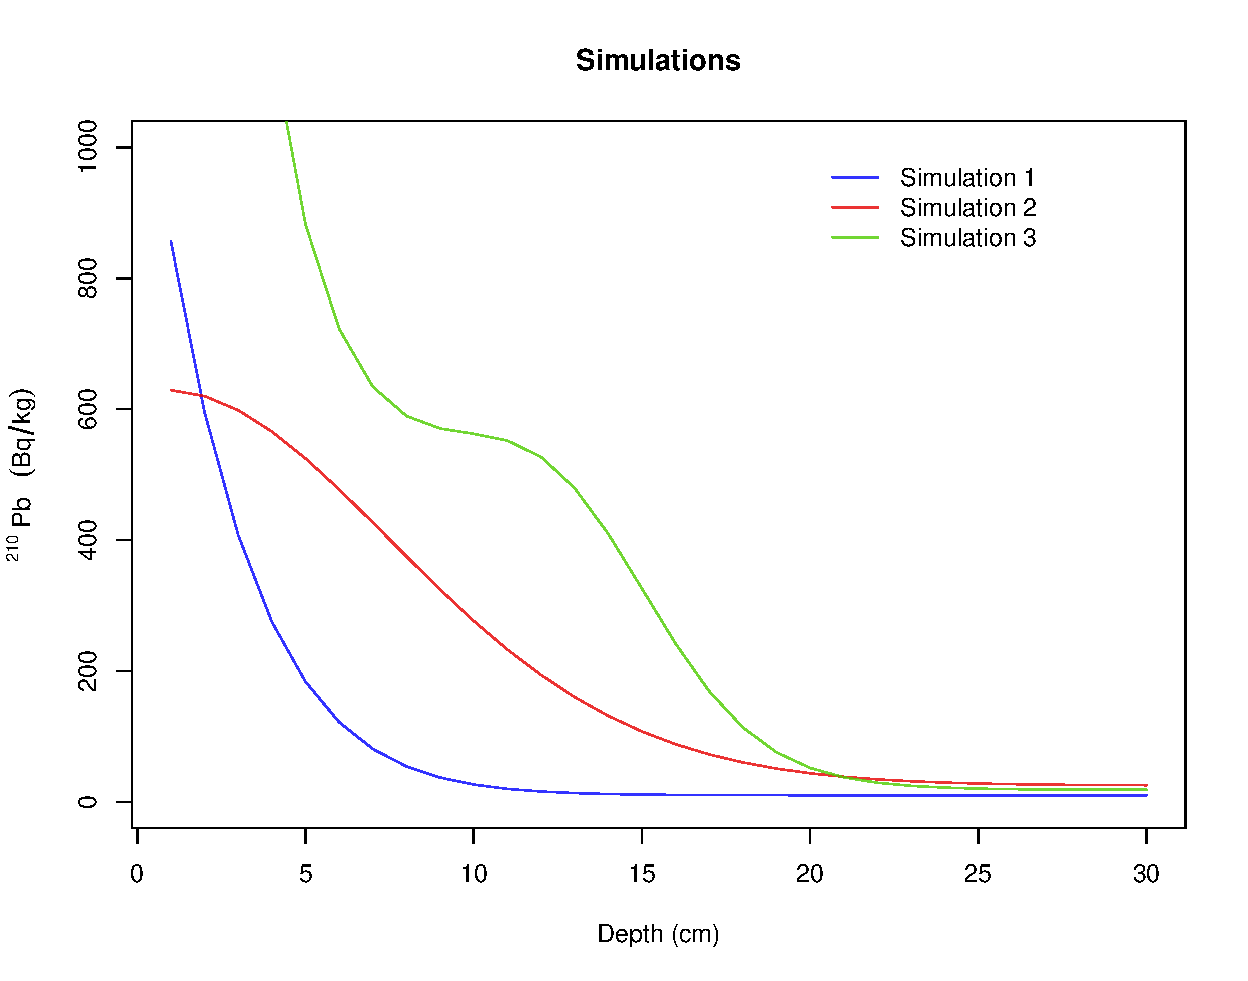
\includegraphics[width=\linewidth]{Simulations_t_act.pdf}
  \caption{Simulated $^{210}Pb$ concentration in relation to depth.}
  \label{fig:true_210}
\end{figure}

	These concentrations can be interpreted as error-free measurements. Because every equipment is subject to error, we need to replicate this measurement errors. \citep{Blaauw2018} presents error structure for radiocarbon dates. We can use this structure to our $^{210}Pb$ measurements as both measurements are subject to similar measurement problems. 

	Let $C_{\hat{x}}$ be the true  $^{210}Pb$ concentration in the interval $\hat{x}=[a,b)$, given the age-depth function $t(x)$. To simulate disturbances in the material, we can introduce scatter centred around the true value, $C\sim \mathcal{N}\left(C_{\hat{x}},x^2_{scat}\right)$, where $x^2_{scat}$ is the amount of scatter for this variable (in this case $x^2_{scat}=10$). Now, to replicate outliers, we define a shift from the true value ($x_{shift}$), which occurs with a probability $p_{out}$. This results in a new variable $\theta'$ which is defined as
\begin{align}
	\theta' = \begin{cases}
			\mathcal{U}(\hat{x} - x_{shift}\theta + x_{shift}), &  p_{out} \\
			\theta, & 1-p_{out}
		\end{cases}.
\end{align}

	To simulate the uncertainty provided by the laboratory, we can define the simulated measurements as  $y(\theta')\sim\mathcal{N}\left(\mu(\theta'),\sigma^2\right)$, where $\sigma_R$ is the standard deviation reported by the laboratory. To simulate $\sigma_R$ we use $\sigma_R= \max \left(\sigma_{min}, \mu(\theta')~\varepsilon~y_{scat}~\right)$, where $\sigma_{min}$ is the minimum standard deviation assigned to a measurement. This variable differs between laboratories (we will be using a default value of $1~ Bq/kg$). Finally, $\varepsilon$ is the analytical uncertainty (default .01) and $y_{scat}$ an error multiplier (default 1.5).

	For this this study we created a data set for each simulation by integrating in intervals of 1 cm from depth 0 to 30 (where equilibrium was guaranteed).The complete data sets can be found in the Supplementary Material \ref{sec:supp_mat} and Figure \ref{fig:true_210} $^{210}Pb$ concentrations curves. 

	With these base data sets, we then define a new variable call percentage of information. This variable relates to how many much of the available information was measured. For this we assumed that background was reached at depth $m$, information percentage is define as how much area of the core was measured, e.g. if background was reached at depth $100$ cm and the core was sampled very $1$ cm if 20 samples are measured, the percentage of information would be 20 \%. This variable will help us to have a measuring tool for how many samples are needed for a good chronology without depending on the size of the samples. 


\section{Model Comparison}

In order to compare both the CRS and Plum under simular circumstances the previously described data sets will be randomly selected for samples given a information percentage, e.g. for a percentage information of 50\% given our 30 sample data set, 14 samples will randomly selected from the samples at depths 1 to 29, and the samples at depth 30 will be always included. This was done to guaranty that background is reached, which is required for the CRS model. In the case of cores which have not reach background, \textit{Plum}  \citep{Aquino2018} has shown to provide accurate results without the need of user interference, the CRS can provide a chronology if inventory is completed, which means user innervation. To avoid this problem and to provide a more objective comparison every sampling set will have reach background.  
\subsection{Sampling Techniques }

In order to observe how sampling affects the accuracy and precision of $^{210}Pb$ models, we used the three simulated data sets created for the previous section. This simulated cores were randomly selected given a percentage of information (e.g. for a 20\% information sample, in the 30 cm cores, 6 random samples were selected). Becase the CRS model assumes that background has being reached, we decided to fix the last sample (30 cm depth) for every case, this will facilitate the CRS to provide more accurate results and also gives the model a single last depth to be removed as it is common practice when using this model. 100 individual samples were selected for information percentage from 10\% to 90\% in a 5\% intervals (e.i 10\%, 15\%, 20\%,...,85\% and 90\%).After a random sample was selected both the CRS model and Plum were performed and compared to the true age value to calculate its accuracy. 

In order to observe the precision and accuracy we decided to calculate the mean of length of the 95\% intervals (in yr), the offset (in yr) as well as the normalized accuracy (this variable will show us how far the model is from the true value given its uncertainty).  


\begin{figure}
 \centering
  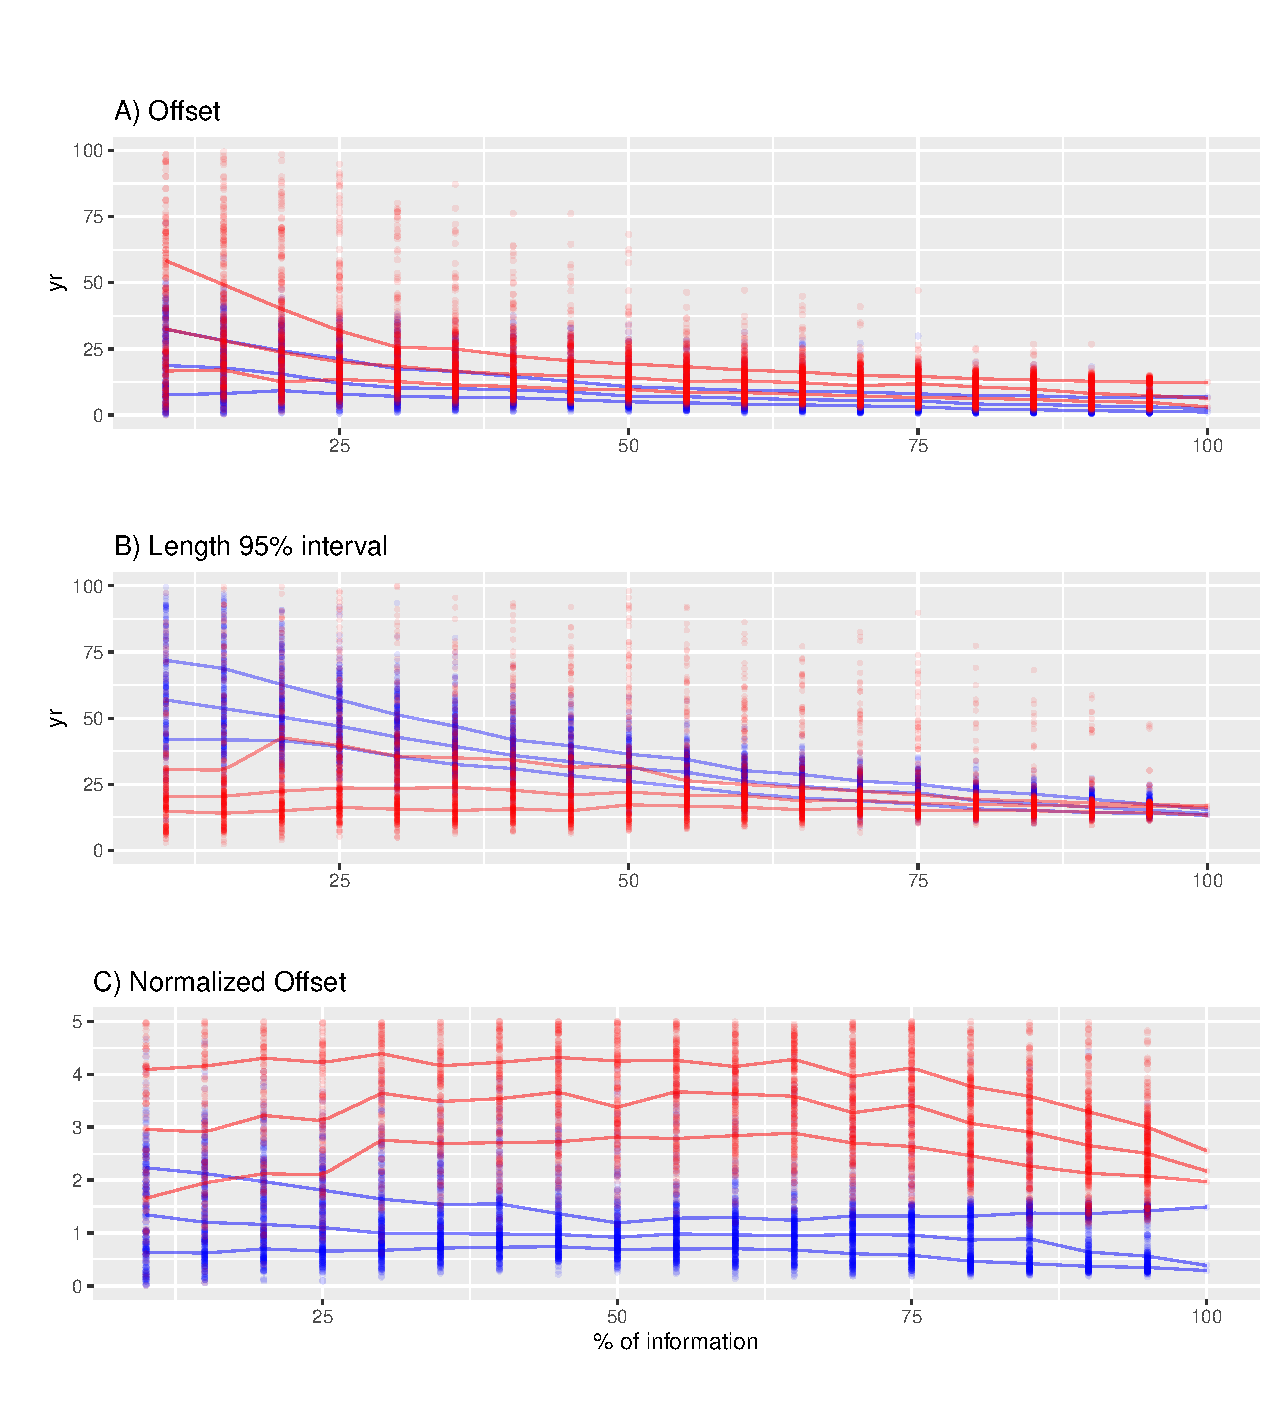
\includegraphics[width=\linewidth]{AccPrec.pdf}
  \caption{}
  \label{fig:accpre}
\end{figure}

From Figure \ref{fig:accpre}, we can observe similar results those presented by \cite{Blaauw2018}. The classical model (CRS) at first appears to provide a similar result (similar offset) to the Bayesian alternative (\textit Plum}) with a more precise results (if we only look at the length of the 95\% interval). 
These results can be misleading if we don't analysed the effects of these two parameters in conjunction (offset and length of interval). In order to observe how well the model captures the true ages calculated the normal offset (see Figure \ref{fig:accpre}). 
These figures shows how on average the models contain the true within their uncertainty intervals (normalized to one standard deviation). Any value which is over the second standard deviations represents that the model is incapable of capturing the true ages within their uncertainty intervals.  
This means that the CRS provides small uncertainties at the cost of its accuracy.
It also appears that the length of the 95\% interval and offset is not affected by how much information is provided to the model. This is a results of the use of interpolation used by the method. 

On the other hand, \textit{Plum}, which is a Bayesian method, shows more accurate results as more information is given to the model, this are similart to the ones found by \citet{Blaauw2018}. 
When we observe the regular offset (not normalized), we observed that Plum provides a much smaller offset in comparison to the CRS model, this in combination with slightly bigger uncertainties results on a consistently accurate model which is capable of capturing the true values within its uncertainty intervals. 
This result supports the clame that \textit{Plum} provides more realistic uncertainties when compared to the CRS. 





\begin{figure}
 \centering
  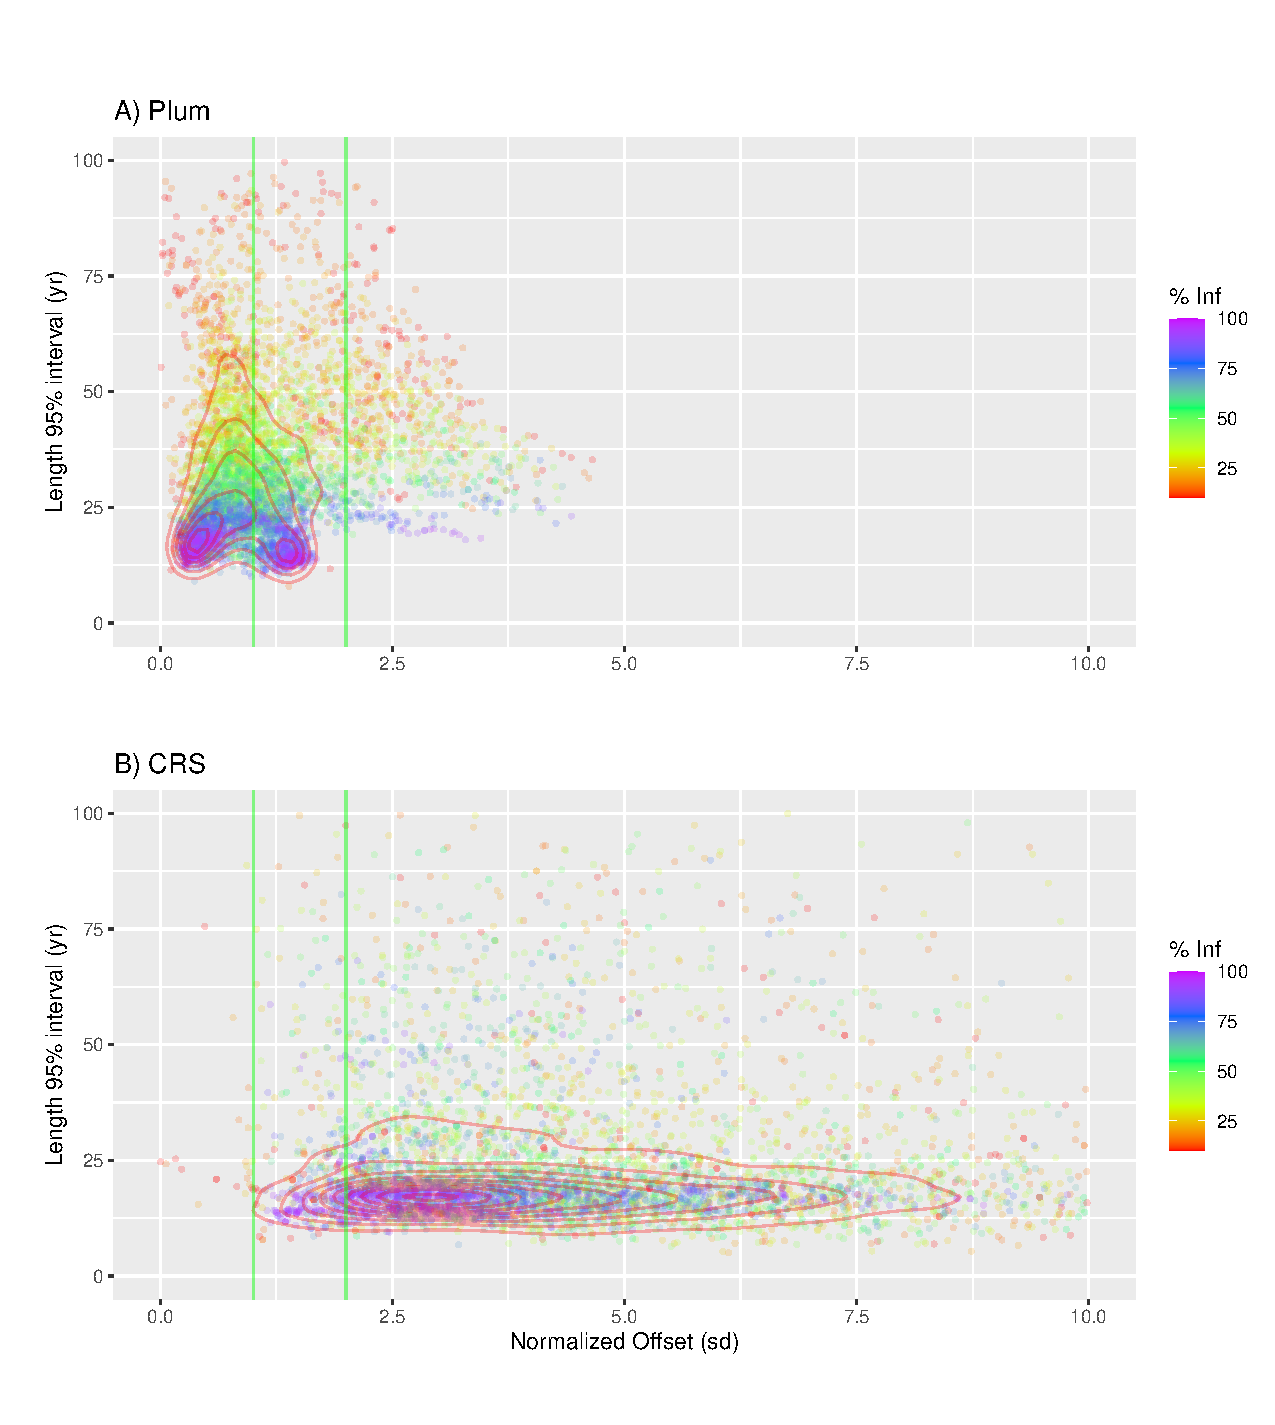
\includegraphics[width=\linewidth]{Maps.pdf}
  \caption{}
  \label{fig:accpre}
\end{figure}

Plum has 87.86\% (4686/5333) of its runs under the 2 standard deviations, on the other hand the CRS model only has 7.48\% (399/5333).
We can also observe a clear structure on the way Plum increases its accuracy and precision to obtained a better chronology, on the side the CRS model appears to not have this structure. 



\newpage


\section{Supplementary Material}
\label{sec:supp_mat}
\newpage
\begin{table}[H]
	\begin{tabular}{c|cllllll}
		Label    & Depth & Density  & 210Pb & sd(210Pb) & Thickness& 226Ra  & sd(226Ra) \\
		& (cm) &($g/cm^3$) &(Bq/kg)& & (cm) & (Bq/kg)&\\
		\hline 
		Sim01-01 & 1          & 0.10009                         & 63.50103      & 2.85755   & 1              & 23.8045       & 1.125     \\
		Sim01-02 & 2          & 0.10064                         & 80.08738      & 3.60393   & 1              & 23.2924       & 1.125     \\
		Sim01-03 & 3          & 0.10173                         & 98.32806      & 4.42476   & 1              & 23.434        & 1.125     \\
		Sim01-04 & 4          & 0.10334                         & 125.45705     & 5.64557   & 1              & 26.0873       & 1.125     \\
		Sim01-05 & 5          & 0.10547                         & 141.27971     & 6.35759   & 1              & 22.8041       & 1.125     \\
		Sim01-06 & 6          & 0.10809                         & 130.27571     & 5.86241   & 1              & 23.4333       & 1.125     \\
		Sim01-07 & 7          & 0.11116                         & 134.04051     & 6.03182   & 1              & 25.6156       & 1.125     \\
		Sim01-08 & 8          & 0.11466                         & 129.69245     & 5.83616   & 1              & 26.1371       & 1.125     \\
		Sim01-09 & 9          & 0.11855                         & 134.93655     & 6.07214   & 1              & 25.4813       & 1.125     \\
		Sim01-10 & 10         & 0.12278                         & 109.39886     & 4.92295   & 1              & 25.8877       & 1.125     \\
		Sim01-11 & 11         & 0.12731                         & 110.68133     & 4.98066   & 1              & 24.4414       & 1.125     \\
		Sim01-12 & 12         & 0.13209                         & 102.38094     & 4.60714   & 1              & 24.9053       & 1.125     \\
		Sim01-13 & 13         & 0.13706                         & 75.80895      & 3.4114    & 1              & 22.9151       & 1.125     \\
		Sim01-14 & 14         & 0.14218                         & 77.60406      & 3.49218   & 1              & 24.4808       & 1.125     \\
		Sim01-15 & 15         & 0.14738                         & 68.4401       & 3.0798    & 1              & 24.9343       & 1.125     \\
		Sim01-16 & 16         & 0.15262                         & 60.72037      & 2.73242   & 1              & 25.2659       & 1.125     \\
		Sim01-17 & 17         & 0.15782                         & 50.28147      & 2.26267   & 1              & 22.961        & 1.125     \\
		Sim01-18 & 18         & 0.16294                         & 44.24641      & 1.99109   & 1              & 22.9139       & 1.125     \\
		Sim01-19 & 19         & 0.16791                         & 39.85997      & 1.7937    & 1              & 28.3774       & 1.125     \\
		Sim01-20 & 20         & 0.17269                         & 38.40823      & 1.72837   & 1              & 23.5379       & 1.125     \\
		Sim01-21 & 21         & 0.17722                         & 32.75922      & 1.47416   & 1              & 25.4363       & 1.125     \\
		Sim01-22 & 22         & 0.18145                         & 28.02545      & 1.26115   & 1              & 24.8995       & 1.125     \\
		Sim01-23 & 23         & 0.18534                         & 27.8749       & 1.25437   & 1              & 22.6783       & 1.125     \\
		Sim01-24 & 24         & 0.18884                         & 30.74797      & 1.38366   & 1              & 24.8575       & 1.125     \\
		Sim01-25 & 25         & 0.19191                         & 28.36187      & 1.27628   & 1              & 24.8724       & 1.125     \\
		Sim01-26 & 26         & 0.19453                         & 27.24535      & 1.22604   & 1              & 24.3778       & 1.125     \\
		Sim01-27 & 27         & 0.19666                         & 23.59236      & 1.06166   & 1              & 24.7209       & 1.125     \\
		Sim01-28 & 28         & 0.19827                         & 25.74855      & 1.15868   & 1              & 24.6615       & 1.125     \\
		Sim01-29 & 29         & 0.19936                         & 25.05368      & 1.12742   & 1              & 24.7199       & 1.125     \\
		Sim01-30 & 30         & 0.19991                         & 25.0065       & 1.12529   & 1              & 24.4937       & 1.125    
	\end{tabular}
\end{table}


\begin{table}[H]
	\begin{tabular}{c|cllllll}
		Label    & Depth& Density& 210Pb & sd(210Pb) & Thickness & 226Ra & sd(226Ra) \\
				& (cm) &($g/cm^3$) &(Bq/kg)& & (cm) & (Bq/kg)&\\
		\hline 
		Sim02-01 & 1          & 0.1001                          & 909.3928      & 40.9227   & 1              & 8.9761        & 0.45      \\
		Sim02-02 & 2          & 0.1006                          & 683.9989      & 30.7799   & 1              & 10.0607       & 0.45      \\
		Sim02-03 & 3          & 0.1017                          & 453.0503      & 20.3873   & 1              & 9.8701        & 0.45      \\
		Sim02-04 & 4          & 0.1033                          & 310.7897      & 13.9855   & 1              & 10.37         & 0.45      \\
		Sim02-05 & 5          & 0.1055                          & 218.0058      & 9.8103    & 1              & 10.0418       & 0.45      \\
		Sim02-06 & 6          & 0.1081                          & 158.6974      & 7.1414    & 1              & 10.104        & 0.45      \\
		Sim02-07 & 7          & 0.1112                          & 113.9062      & 5.1258    & 1              & 10.2049       & 0.45      \\
		Sim02-08 & 8          & 0.1147                          & 75.5493       & 3.3997    & 1              & 9.334         & 0.45      \\
		Sim02-09 & 9          & 0.1185                          & 56.6252       & 2.5481    & 1              & 10.5145       & 0.45      \\
		Sim02-10 & 10         & 0.1228                          & 44.1595       & 1.9872    & 1              & 9.8677        & 0.45      \\
		Sim02-11 & 11         & 0.1273                          & 34.7448       & 1.5635    & 1              & 9.7694        & 0.45      \\
		Sim02-12 & 12         & 0.1321                          & 25.384        & 1.1423    & 1              & 10.5134       & 0.45      \\
		Sim02-13 & 13         & 0.1371                          & 24.0007       & 1.08      & 1              & 10.4589       & 0.45      \\
		Sim02-14 & 14         & 0.1422                          & 21.3643       & 1         & 1              & 9.9504        & 0.45      \\
		Sim02-15 & 15         & 0.1474                          & 17.7932       & 1         & 1              & 10.5135       & 0.45      \\
		Sim02-16 & 16         & 0.1526                          & 15.0416       & 1         & 1              & 10.3362       & 0.45      \\
		Sim02-17 & 17         & 0.1578                          & 14.2937       & 1         & 1              & 10.5131       & 0.45      \\
		Sim02-18 & 18         & 0.1629                          & 12.3844       & 1         & 1              & 10.368        & 0.45      \\
		Sim02-19 & 19         & 0.1679                          & 12.6023       & 1         & 1              & 10.5297       & 0.45      \\
		Sim02-20 & 20         & 0.1727                          & 11.9329       & 1         & 1              & 10.0924       & 0.45      \\
		Sim02-21 & 21         & 0.1772                          & 9.301         & 1         & 1              & 10.118        & 0.45      \\
		Sim02-22 & 22         & 0.1815                          & 10.7777       & 1         & 1              & 10.249        & 0.45      \\
		Sim02-23 & 23         & 0.1853                          & 12.9491       & 1         & 1              & 10.134        & 0.45      \\
		Sim02-24 & 24         & 0.1888                          & 10.6571       & 1         & 1              & 10.1151       & 0.45      \\
		Sim02-25 & 25         & 0.1919                          & 9.6297        & 1         & 1              & 9.6608        & 0.45      \\
		Sim02-26 & 26         & 0.1945                          & 8.4331        & 1         & 1              & 8.7821        & 0.45      \\
		Sim02-27 & 27         & 0.1967                          & 10.4921       & 1         & 1              & 9.8995        & 0.45      \\
		Sim02-28 & 28         & 0.1983                          & 11.135        & 1         & 1              & 9.2481        & 0.45      \\
		Sim02-29 & 29         & 0.1994                          & 10.109        & 1         & 1              & 10.4398       & 0.45      \\
		Sim02-30 & 30         & 0.1999                          & 9.5404        & 1         & 1              & 10.1114       & 0.45     
	\end{tabular}
\end{table}



\begin{table}[H]
	\begin{tabular}{c|cllllll}
		Label    & Depth & Density & 210Pb & sd(210Pb) & Thickness & 226Ra   & sd(226Ra) \\
						& (cm) &($g/cm^3$) &(Bq/kg)& & (cm) & (Bq/kg)&\\
		\hline 
		Sim03-01 & 1     & 0.1001  & 6384.1354     & 287.2861  & 1         & 15.8007 & 0.675     \\
		Sim03-02 & 2     & 0.1006  & 3550.0809     & 159.7536  & 1         & 14.5245 & 0.675     \\
		Sim03-03 & 3     & 0.1017  & 1954.5702     & 87.9557   & 1         & 15.6527 & 0.675     \\
		Sim03-04 & 4     & 0.1033  & 1183.8917     & 53.2751   & 1         & 14.5175 & 0.675     \\
		Sim03-05 & 5     & 0.1055  & 760.2132      & 34.2096   & 1         & 14.9242 & 0.675     \\
		Sim03-06 & 6     & 0.1081  & 360.2553      & 16.2115   & 1         & 14.801  & 0.675     \\
		Sim03-07 & 7     & 0.1112  & 212.9402      & 9.5823    & 1         & 14.8738 & 0.675     \\
		Sim03-08 & 8     & 0.1147  & 104.2684      & 4.6921    & 1         & 14.9028 & 0.675     \\
		Sim03-09 & 9     & 0.1185  & 44.3849       & 1.9973    & 1         & 15.0768 & 0.675     \\
		Sim03-10 & 10    & 0.1228  & 18.6447       & 1         & 1         & 15.3764 & 0.675     \\
		Sim03-11 & 11    & 0.1273  & 23.2778       & 1.0475    & 1         & 14.6231 & 0.675     \\
		Sim03-12 & 12    & 0.1321  & 53.1587       & 2.3921    & 1         & 15.1629 & 0.675     \\
		Sim03-13 & 13    & 0.1371  & 97.363        & 4.3813    & 1         & 14.3047 & 0.675     \\
		Sim03-14 & 14    & 0.1422  & 116.9788      & 5.264     & 1         & 14.0261 & 0.675     \\
		Sim03-15 & 15    & 0.1474  & 153.2901      & 6.8981    & 1         & 15.9723 & 0.675     \\
		Sim03-16 & 16    & 0.1526  & 151.8496      & 6.8332    & 1         & 14.7579 & 0.675     \\
		Sim03-17 & 17    & 0.1578  & 136.3609      & 6.1362    & 1         & 16.114  & 0.675     \\
		Sim03-18 & 18    & 0.1629  & 107.2736      & 4.8273    & 1         & 15.4595 & 0.675     \\
		Sim03-19 & 19    & 0.1679  & 76.8966       & 3.4603    & 1         & 15.9439 & 0.675     \\
		Sim03-20 & 20    & 0.1727  & 48.9213       & 2.2015    & 1         & 14.6235 & 0.675     \\
		Sim03-21 & 21    & 0.1772  & 40.4439       & 1.82      & 1         & 14.6716 & 0.675     \\
		Sim03-22 & 22    & 0.1815  & 26.5638       & 1.1954    & 1         & 16.2541 & 0.675     \\
		Sim03-23 & 23    & 0.1853  & 21.714        & 1         & 1         & 14.4826 & 0.675     \\
		Sim03-24 & 24    & 0.1888  & 17.6428       & 1         & 1         & 15.5109 & 0.675     \\
		Sim03-25 & 25    & 0.1919  & 17.3533       & 1         & 1         & 13.6898 & 0.675     \\
		Sim03-26 & 26    & 0.1945  & 17.4211       & 1         & 1         & 14.4684 & 0.675     \\
		Sim03-27 & 27    & 0.1967  & 16.4246       & 1         & 1         & 15.3889 & 0.675     \\
		Sim03-28 & 28    & 0.1983  & 12.4828       & 1         & 1         & 15.0698 & 0.675     \\
		Sim03-29 & 29    & 0.1994  & 13.5514       & 1         & 1         & 15.2346 & 0.675     \\
		Sim03-30 & 30    & 0.1999  & 14.3145       & 1         & 1         & 14.7846 & 0.675    
	\end{tabular}
\end{table}


\bibliographystyle{apalike}
\bibliography{bibliography.bib}

\end{document}
